% ----------- 1. DECLARACIÓN DE CLASE Y OPCIONES -----------
\documentclass[acmsmall, screen=true, review=false]{acmart}

% 'acmsmall': Define el formato de columna simple para journals.
% 'screen=true': Habilita enlaces de colores para visualización en pantalla.
% 'review=false': Deshabilita el modo de revisión (numeración de líneas).

% ----------- 2. PAQUETES (El sistema ACM los carga automáticamente) -----------
\usepackage{tikz} %para graficas
\usetikzlibrary{arrows.meta, positioning, calc, decorations.pathreplacing}
\usepackage{cancel}

% Si usas BibTeX, asegúrate de que use el estilo de citas de ACM (por defecto).
\citestyle{acmnumeric} % Opcional, pero define el estilo de citas (numérico).

% ----------- 3. METADATOS (TOP MATTER) -----------
\acmJournal{TOS} % Reemplaza con la abreviatura real de tu revista ACM
\acmVolume{1}
\acmNumber{1}
\acmArticle{1} %que onda con esto?
\acmYear{2025}
\acmMonth{11} % 11 para noviembre
\setcopyright{acmlicensed}

\title[Teoremas de Jerarquía]{Teoremas de Jerarquía}
\subtitle{Seccion 9.1 Indroducción a la Teoría de la Computación, Michael Sipser}

% Autor 1
\author{Ana Sofía Hernández Zavala}
%\orcid{319316717}
\affiliation{
  \institution{Universidad Nacional Autónoma de México, Facultad de Ciencias}
  \city{Ciudad de México}
  \country{México} % OBLIGATORIO
}
\email{anasofiahdzz@ciencias.unam.mx}

% Autor 2
\author{Nombre del Autor 2}
\affiliation{
  \institution{Otra Universidad/Departamento}
  \city{Otra Ciudad}
  \country{Otro País}
}
\email{autor2@ejemplo.com}

% Autor 3
\author{Nombre del Autor 3}
\affiliation{
  \institution{Otra Universidad/Departamento}
  \city{Otra Ciudad}
  \country{Otro País}
}
\email{autor2@ejemplo.com}

%checar esto
% Conceptos de Clasificación de Computación ACM (CCS)
% Obligatorio para artículos > 2 páginas.
\begin{CCSXML}
<ccs2012>
 <concept>
  <concept_id>10003033.10003083.10003095</concept_id>
  <concept_desc>Networks~Network reliability</concept_desc>
  <concept_significance>500</concept_significance>
 </concept>
</ccs2012>
\end{CCSXML}

\ccsdesc[500]{Networks~Network reliability}

% Palabras clave (Keywords)
\keywords{teoremas, jerarquías, tiempo, espacio, corolario, definicion, máquina de Turing}

% ----------- 4. COMIENZO DEL DOCUMENTO -----------
\begin{document}

% 1. EL RESUMEN VA PRIMERO, DENTRO DE begin{document}
\begin{abstract}
Este es el resumen de la investigación. (Ya puedes borrar el comentario confuso que estaba aquí).
\end{abstract}

% 2. LUEGO SE GENERA EL BLOQUE DE TÍTULO Y METADATOS
\maketitle

% 3. LUEGO VIENE LA PRIMERA SECCIÓN
\section{Introducción}
El sentido común nos dice que si le damos más tiempo o más espacio a una máquina de Turing entonces debería de incrementar la clase de problemas que podría resolver; y los Teoremas de Jerarquía lo confirman, ya que estos teoremas prueban que las clases de complejidad de tiempo y espacio no son todas las mismas. \\
Por ejemplo en este articulo mostraremos que el teorema de jerarquía de complejidad del espacio es más simple que el del tiempo.

\section{Teorema del Espacio}
\begin{definition}
    Una función $f: N \rightarrow N $, donde $f(n)$ es al menos $O(log_n)$, es llamada espacio constructible si la funcion que mapea la cadena de $1^n$ a la representación binaria de $f(n)$ es computada en espacio $O(f(n))$. \cite{cita1}
\end{definition}
Es decir que $f$ es un espacio constructible si alguna máquina de Turing M de tiempo $O(f(n))$ existe y siempre se detiene con la representacion binaria de $f(n)$ en su cinta cuando empieza en la entrada $1^n$. \cite{cita1}.
Se encontró una mejora significativa.\\
El rol del espacio constructible en el teorema de jerarquía del espacio se entiende mejor de la siguiente manera: Si se tiene un $f(n)$ que es mayor o un poco más grande que $g(n)$ en espacio, entonces $f(n)$ debería de poder analizar más lenguajes, pero supongamos que $f(n)$ esta analizando un lenguaje muy grande entonces ocupa todo el espacio sobrante o incluso requerirá más espacio del diponible.\\
Es así como llegamos al teorema formal de la jerarquía del espacio.
\begin{theorem}
  Para cualquier función $f:N \rightarrow N$ del espacio constructible, existe un lenguaje $A$ que es decidible en espacio $O(f(n))$ pero no en espacio $o(f(n))$.
  \label{thm:Teorema de la jerarquía del espacio} \cite{cita1}
\end{theorem}
La prueba a lo anterior es básicamente demostrar que el lenguaje $A$ tiene 2 propiedades:
\begin{itemize}
  \item $A$ es decidible en espacio $O(f(n))$.
  \item $A$ no es decidible en espacio $o(f(n))$.
\end{itemize} 
Describiendo a $A$ con un algoritmo $D$ que lo decide, $D$ corre en espacio $O(f(n))$, así cumple con la primer propiedad; y $D$ garantiza que $A$ es diferente de cualquier lenguaje que es decidible en espacio $o(f(n))$, lo cual asegura la segunda propiedad. \\
Esto dado a
\begin{corollary}
  Para cualesquiera 2 funciones $f_1, f_2: N \rightarrow N$, donde $f_1(n)$ es $o(f_2(n))$ y $f_2$ es espacio constructible, $SPACE(f_1(n)) \subsetneq SPACE(f_2(n))$. \cite{cita1}
\end{corollary}
En otras palabras, \textit{SPACE}$(o(f(n))) \subsetneq$ \textit{SPACE}$(f(n))$, siendo \textit{SPACE(o(f(n)))=} \textit{\{B $|$ alguna maquina de Turing M que decide B en espacio o(f(n))\}} \cite{cita2}\\
%lo anterior viene de un corolario del libro
%imagen1 notas
\begin{figure}[h!] 
    \centering 
    
    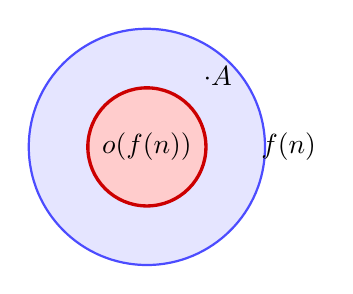
\begin{tikzpicture}
        \draw[
            thick,
            blue!70,
            fill=blue!10
        ] (0, 0) circle (1.5cm);
        
        \node at (1.8, 0) {$f(n)$};
        
        \draw[
            very thick,
            red!80!black,
            fill=red!20
        ] (0, 0) circle (0.75cm);
        
        \node at (0.9, 0.9) {$\cdot A$}; 
        
        \node at (0, 0) {$o(f(n))$}; 
    \end{tikzpicture}
    
    \caption{\textit{SPACE}$(o(f(n))) \subsetneq$ \textit{SPACE}$(f(n))$.}
    \label{fig:subconjunto} 
\end{figure}

Parecido a la situación de un lenguaje libre de contexto, en el caso de los lenguajes regulares, donde se muestra un lenguaje particular que se diferencía por ser libre de contexto pero no regular.\\
Usando la prueba de diagonalización, se construye una máquina de Turing $D$ que decide el lenguaje $A$ con las siguientes propiedades:
\begin{enumerate}
  \item $D$ generará el lenguaje $A$.
  \item $D$ se ejecutará dentro de $f(n)$.
  \item $D$ se diseñará para asegurarse que su lenguaje no pueda implementarse en un espacio menor, para eso se asegura que su lenguaje sea diferente de cualquier lenguaje decidible por una máquina de Turing en un espacio menor.
  \item $D$ se asegurará que no puede ser implementada en $o(f(n))$.
\end{enumerate}

Prueba: Dada una máquina de Turing D donde:
\begin{enumerate}
  \item $D$ corre en espacio $O(f(n))$.
  \item $D$ es cierto que $L(D) \neq L(M)$ para cualquier MT M que corra en espacio $o(f(n))$.
  \item Dejar $A = L(D)$.
\end{enumerate}

El objetivo de esto es mostrar que $A \in SPACE(f(n))$ pero $A \notin SPACE(o(f(n)))$.
\begin{enumerate}
  \item $D$ recibe como entrada $w$
  \item Marcar las celdas de la cinta $f(n)$ donde $n=|w|$; si trata de usar más cinta, rechaza (solo se permitirá que use el espacio $f(n)$ de lo contrario tal vez D no este en $f(n)$). Para asegurarnos de que eso no pase entonces se coloca el $\#$ para delimitar el espacio $f(n)$, si trata de usar más que eso, rechaza.
  \item Si $w \neq <M>$ para alguna máquina de Turing M, rechazar (w no describe nada, solo es un salto). Rechaza a menos que si sea una $w$ que describa una maquina de Turing M.
  %imagen de la cinta 
  \item Simular * $M$ en $w$.\\ Acepta si M rechaza.\\ Rechaza si M acepta.\\ *NOTA: $D$ puede simular $M$ con un factor constante de espacio.
\end{enumerate}
  %imagen de la cinta 
\begin{figure}[h!]
    \centering
    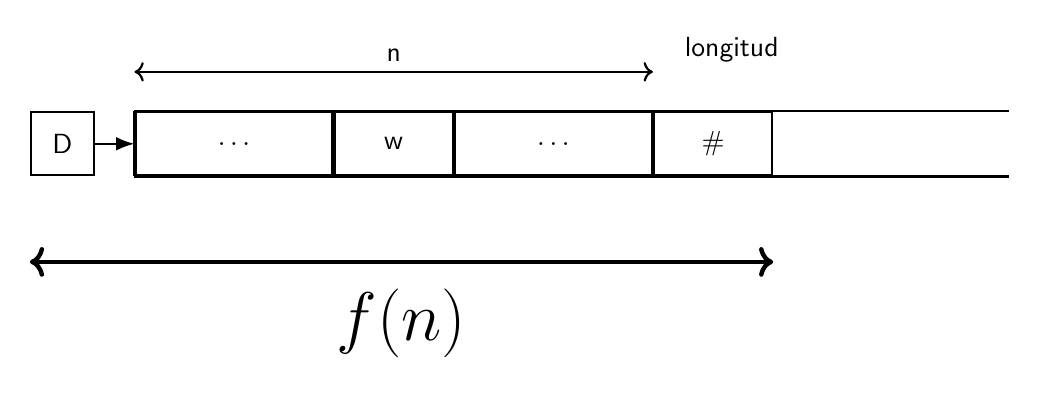
\begin{tikzpicture}[
        every node/.style={font=\sffamily}, % Estilo para todo el texto: sans-serif.
        box/.style={draw=black, thick, rectangle, minimum width=0.8cm, minimum height=0.8cm}, 
        tape/.style={draw=black, thick, rectangle, minimum height=0.8cm}, 
        arrow_style/.style={-Latex, thick, draw=black} 
    ]
        % --- Caja D ---
        \node[box] (D) at (-2,0) {D};

        % --- Celdas de Contenido (Con sus propias cajas y bordes internos) ---
        \node[tape, minimum width=2.5cm, right=0.5cm of D.east, anchor=west] (dots1) {$\dots$};
        \node[tape, minimum width=1.5cm, right=0cm of dots1.east, anchor=west] (w_cell) {w};
        \node[tape, minimum width=2.5cm, right=0cm of w_cell.east, anchor=west] (dots2) {$\dots$};
        \node[tape, minimum width=1.5cm, right=0cm of dots2.east, anchor=west] (hash_cell) {\#};

        % --- Cinta "Abierta" y Larga (Extensión) ---
        
        % 1. Dibujamos la línea de contorno normal, pero solo hasta el borde derecho de la celda #
        %    *NO* usamos 'rectangle', sino líneas individuales.
        \coordinate (tape_north_west) at (dots1.north west);
        \coordinate (tape_south_west) at (dots1.south west);
        \coordinate (tape_north_east_content) at (hash_cell.north east);
        \coordinate (tape_south_east_content) at (hash_cell.south east);

        % 2. Extendemos el borde derecho 3cm más allá de hash_cell.east
        \coordinate (extended_east_north) at ($(hash_cell.north east) + (3cm, 0)$);
        \coordinate (extended_east_south) at ($(hash_cell.south east) + (3cm, 0)$);

        % Dibujamos las líneas:
        % (a) Línea superior: desde el inicio hasta el final extendido
        \draw[thick, draw=black] (tape_north_west) -- (extended_east_north); 
        % (b) Línea inferior: desde el inicio hasta el final extendido
        \draw[thick, draw=black] (tape_south_west) -- (extended_east_south); 
        
        % Esto es crucial: dibuja la línea izquierda que fue omitida por las celdas
        \draw[thick, draw=black] (tape_north_west) -- (tape_south_west);
        
        % ¡OJO!: Las líneas divisorias internas están dadas por el estilo 'tape' de cada nodo.

        % --- Flecha de D a la cinta ---
        \draw[arrow_style] (D.east) -- (dots1.west); 

        % --- Longitud n ---
        \path let \p1 = (dots1.north west), \p2 = (dots2.north east) in
              coordinate (n_start) at (\x1, \y1)
              coordinate (n_end) at (\x2, \y2);
            
        \draw[<->, thick, draw=black] ($(n_start) + (0, 0.5cm)$) 
            -- node[above, font=\sffamily] {n} 
            ($(n_end) + (0, 0.5cm)$)
            node[above, xshift=1cm, font=\sffamily] {longitud}; 

        % --- f(n) (RECTA y TERMINANDO EN #) ---
        
        \coordinate (fn_start_point) at ($(D.west) - (0, 1.5cm)$); 
        % Usamos la coordenada X de hash_cell.east y la Y de fn_start_point para asegurar la rectitud
        \coordinate (fn_end_point) at (hash_cell.east |- fn_start_point); 
            
        \draw[<->, ultra thick, draw=black] (fn_start_point)
            -- node[below=0.2cm, font=\sffamily\bfseries\Huge] {$f(n)$} (fn_end_point); 
            
    \end{tikzpicture}
    \caption{Punto 1. Solo se permitirá que D use el espacio f(n), de lo contrario tal vez D no este en f(n).}
    \label{fig:turing_tape_final_completo}
\end{figure}

$D$ está haciendo algo diferente a $A$, $D$ no puede ser diferente de cada $M$ porque $D$ en sí misma es una máquina de Turing, $D$ solo se ejecuta dentro de celdas $f(n)$ de la cinta, tiene que poder realizar esa simulación de M dentro de esa cantidad de cinta, siempre rechazará si usa más.\\
Si $M$ usa menos que $D$, entonces puede hacer la simulación.
\subsection{Problemas}
\subsubsection{¿Qué pasa si M corre en tiempo o(f(n)) pero tiene una constante grande?}
Entonces $D$ no tendrá espacio para simular $M$ cuando es pequeña.\\
\textit{Solución:} Simular $M$ en infinitos $w's$. Pensando en $w$ como la representación de $M$ pero con un número ilimitado de ceros finales. Se cambia el punto $3.$ por $3. Si w \neq <M>10^*$ por alguna máquina de Turing M, rechaza.\\ Lo primero que se hará con $w$ es eliminar los ceros finales hasta el último 1 y tomar el resto como la descripción de la máquina. Si $M$ de verdad esta corriendo en $o(f(n))$ entoces habrá espacio suficiente para que $M$ se ejecute completamente sobre $w$ y así diferenciarlo de él.\\
%imagen de la cinta
\begin{figure}[h!]
    \centering
    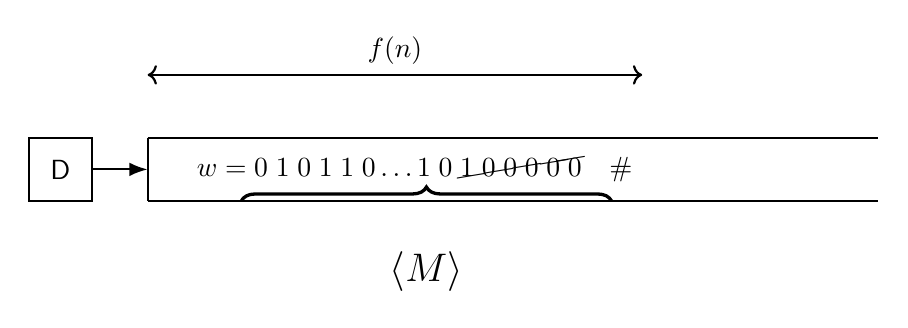
\begin{tikzpicture}[
        every node/.style={font=\sffamily},
        box/.style={draw=black, thick, rectangle, minimum width=0.8cm, minimum height=0.8cm}, 
        arrow_style/.style={-Latex, thick, draw=black} 
    ]
        % --- Caja D ---
        \node[box] (D) at (-2,0) {D};

        % --- Cinta Principal (Contenido y Coordenadas) ---
        \node[font=\sffamily] (content) at (2.5, 0) {$w = 0\; 1\; 0\; 1\; 1\; 0 \dots 1\; 0\; \cancel{1\; 0\; 0\; 0\; 0\; 0}  \quad \#$};
        
        \def\tapeHeight{0.4cm}
        \def\extensionLength{3cm} 

        \coordinate (content_west) at (content.west);
        \coordinate (content_east) at (content.east);

        % Puntos de inicio y fin de la cinta
        \coordinate (tape_start_top) at ($(content_west) + (-0.5cm, \tapeHeight)$);
        \coordinate (tape_start_bottom) at ($(content_west) + (-0.5cm, -\tapeHeight)$);
        
        % Puntos del final extendido de la cinta
        \coordinate (tape_end_top) at ($(content_east) + (\extensionLength, \tapeHeight)$);
        \coordinate (tape_end_bottom) at ($(content_east) + (\extensionLength, -\tapeHeight)$);
        
        % Dibujamos las líneas de la cinta (rectas, sin líneas internas)
        \draw[thick, draw=black] (tape_start_top) -- (tape_start_bottom); % Línea vertical izquierda
        \draw[thick, draw=black] (tape_start_top) -- (tape_end_top);     % Línea superior (recta)
        \draw[thick, draw=black] (tape_start_bottom) -- (tape_end_bottom); % Línea inferior (recta)

        % --- Flecha de D a la cinta ---
        \draw[arrow_style] (D.east) -- (tape_start_top |- D.east); 

        % --- f(n) (RECTA y DESENCIMADA) ---
        \def\fnHeight{0.8cm}
        
        \coordinate (fn_start_point) at ($(tape_start_top) + (0, \fnHeight)$); 
        \coordinate (fn_end_point) at ($(content_east) + (0, \fnHeight + \tapeHeight)$); 
        
        \draw[<->, thick, draw=black] (fn_start_point)
            -- node[above, font=\sffamily] {$f(n)$} (fn_end_point);

        % --- Codificación <M> (ARCO INFERIOR, AJUSTADO AL RANGO 0...0) ---
        
        % COORDENADAS AJUSTADAS para abarcar el código binario
        \coordinate (M_start) at (0.3, 0); % Inicia justo antes del primer '0'
        \coordinate (M_end) at (5.0, 0);   % Termina justo después del último '0'
        
        % Dibuja el corchete curvo (brace) y la etiqueta
        \draw[decorate, decoration={brace, amplitude=5pt, mirror}, very thick] 
            (M_end |- tape_start_bottom) -- (M_start |- tape_start_bottom) 
            node[midway, below=0.5cm, font=\Large] {$\langle M \rangle$};
            
    \end{tikzpicture}
    \caption{Problema 2.2.1 <M> abarca desde el primer 0 hasta el último 0, y se debe de tachar desde el último 0 hasta el último 1.}
    \label{fig:codificacion_m_final_perfecto}
\end{figure}

Ahora $M$ se ejecuta en una gran entrada, suficientemente grande para que $D$ (que tiene más espacios) pueda ejecutarse completamente vacía.
\subsubsection{¿Qué pasa si M se cicla?} D debe detenerse.
Solución: Detener $M$ si corre en $2^{f(n)}$ pasos.\\
*Modificando el paso 4. por 4. Simular * $M$ en $w$ por $2^{f(n)}$ pasos. Acepta si M rechaza. Rechaza si M acepta o no se ha detenido.
\subsubsection{¿Cómo computar f?} $f$ tiene que ser computable dentro del espacio.\\
Solución: Asumir que $f$ es un espacio constructible, i.e. puede computar $f$ con $O(f(n))$. Ciertas funciones como $log_n, log^2_n, n, n^2, 2^n,...$ son espacios constructibles.\\ ¿Se puede decir que $D$ tiene como entrada $M$ y simula $M$ sobre sí mismo? Cierto.

\section{Teorema del Tiempo}

\section{Teorema3}

\section{Conclusiones}
Resumimos nuestros hallazgos aquí.


% ----------- 5. BIBLIOGRAFÍA -----------
\bibliographystyle{ACM-Reference-Format}
\bibliography{referencias} % Llama al archivo referencias.bib

\end{document}